\documentclass[a4paper]{article}
%\documentclass[a4paper,fontsize=13pt]{scrartcl}

\usepackage{vntex}
%\usepackage{helvet} %set font Helvetica

%\usepackage{times} %set font Times New Roman
\renewcommand{\familydefault}{\sfdefault} %set font Sans Serif

%\usepackage[english,vietnam]{babel}
%\usepackage[utf8]{inputenc}

%\usepackage[utf8]{inputenc}
%\usepackage[francais]{babel}
\usepackage{a4wide,amssymb,epsfig,latexsym,array,hhline,fancyhdr}

\usepackage{amsmath}
\usepackage{amsthm}
\usepackage{multicol,longtable,amscd}
\usepackage{diagbox}%Make diagonal lines in tables
\usepackage{booktabs}
\usepackage{alltt}
\usepackage[framemethod=tikz]{mdframed}% For highlighting paragraph backgrounds
\usepackage{caption,subcaption}

\usepackage{lastpage}
\usepackage[lined,boxed,commentsnumbered]{algorithm2e}
\usepackage{enumerate}
\usepackage{color}
\usepackage{graphicx}							% Standard graphics package
\usepackage{array}
\usepackage{tabularx, caption}
\usepackage{multirow}
\usepackage{multicol}
\usepackage{rotating}
\usepackage{graphics}
\usepackage{geometry}

\usepackage{setspace}
%\singlespacing
%\onehalfspacing
%\doublespacing
%\setstretch{1.5}



\usepackage{epsfig}
\usepackage{tikz}
\usetikzlibrary{calc}
\newcommand\HRule{\rule{\textwidth}{1pt}}
\usetikzlibrary{arrows,snakes,backgrounds}
\usepackage[unicode]{hyperref}
\hypersetup{urlcolor=blue,linkcolor=black,citecolor=black,colorlinks=true}
%\usepackage{pstcol} 								% PSTricks with the standard color package

\usepackage{a4wide,amssymb,epsfig,latexsym,array,hhline,fancyhdr}

\usepackage[makeroom]{cancel}
\usepackage{amsmath}
\usepackage{amsthm}
\usepackage{multicol,longtable,amscd}
\usepackage{diagbox}%Make diagonal lines in tables
\usepackage{booktabs}
\usepackage{alltt}
\usepackage[framemethod=tikz]{mdframed}% For highlighting paragraph backgrounds
\usepackage{caption,subcaption}
\usepackage{arydshln}
\usepackage{tabularx} % in the preamble

\setlength\dashlinedash{1.5pt}
\setlength\dashlinegap{4.5pt}
\setlength\arrayrulewidth{0.2pt}

\usepackage{textcomp}
\usepackage{listings}
\usepackage{listingsutf8}
% Typesetting Listings
\usepackage{xcolor}
\usepackage{color}
\definecolor{listinggray}{gray}{0.9}
\definecolor{lbcolor}{rgb}{0.9,0.9,0.9}
\definecolor{Darkgreen}{rgb}{0.1,0.6,0.1}

\lstset{
	backgroundcolor=\color{lbcolor},
	tabsize=4,
	%   rulecolor=,
	language=[GNU]C++,
	basicstyle=\scriptsize,
	upquote=true,
	aboveskip={1.5\baselineskip},
	columns=fixed,
	showstringspaces=false,
	extendedchars=false,
	breaklines=true,
	prebreak = \raisebox{0ex}[0ex][0ex]{\ensuremath{\hookleftarrow}},
	frame=single,
	numbers=left,
	showtabs=false,
	showspaces=false,
	showstringspaces=false,
	identifierstyle=\ttfamily,
	keywordstyle=\color[rgb]{0,0,1},
	commentstyle=\color[rgb]{0.026,0.112,0.095},
	stringstyle=\color[rgb]{0.627,0.126,0.941},
	numberstyle=\color[rgb]{0.205, 0.142, 0.73},
	%        \lstdefinestyle{C++}{language=C++,style=numbers}’.
}
\lstset{
	backgroundcolor=\color{lbcolor},
	tabsize=4,
	language=C++,
	captionpos=b,
	tabsize=3,
	frame=lines,
	numbers=left,
	numberstyle=\tiny,
	numbersep=5pt,
	breaklines=true,
	showstringspaces=false,
	basicstyle=\footnotesize,
	%  identifierstyle=\color{magenta},
	keywordstyle=\color[rgb]{0,0,1},
	commentstyle=\color{Darkgreen},
	stringstyle=\color{red}
}

\usepackage{lastpage}
\usepackage[lined,boxed,commentsnumbered]{algorithm2e}
\usepackage{enumerate}
\usepackage{color}
\usepackage{graphicx}							% Standard graphics package
\usepackage{array}
\usepackage{tabularx, caption}
\usepackage{multirow}
\usepackage{multicol}
\usepackage{rotating}
\usepackage{graphics}
\usepackage{geometry}
\usepackage{setspace}
\usepackage{epsfig}
\usepackage{tikz}
\usetikzlibrary{arrows,snakes,backgrounds}
\usepackage[unicode]{hyperref}
\hypersetup{urlcolor=blue,linkcolor=black,citecolor=black,colorlinks=true}
%\usepackage{pstcol} 								% PSTricks with the standard color package
\usepackage{verbatim}




%\usepackage{fancyhdr}
\setlength{\headheight}{40pt}
\pagestyle{fancy}
\fancyhead{} % clear all header fields
\fancyhead[L]{
 \begin{tabular}{rl}
	\begin{tabular}{l}
		\textbf{\bf \ttfamily Trường ĐH Bách Khoa TP. HCM -- Khoa Khoa học và Kỹ thuật Máy tính}\\
	\end{tabular}
 \end{tabular}
}
\fancyhead[R]{
	\begin{tabular}{l}
		\tiny \bf \\
		\tiny \bf
	\end{tabular}  }
\fancyfoot{} % clear all footer fields
\fancyfoot[L]{\scriptsize \ttfamily Báo cáo Bài tập lớn, môn Lập trình hướng đối tượng}
\fancyfoot[R]{\scriptsize \ttfamily Trang {\thepage}/\pageref{LastPage}}
\renewcommand{\headrulewidth}{0.3pt}
\renewcommand{\footrulewidth}{0.3pt}


%%%
\setcounter{secnumdepth}{4}
\setcounter{tocdepth}{3}
\makeatletter
\newcounter {subsubsubsection}[subsubsection]
\renewcommand\thesubsubsubsection{\thesubsubsection .\@alph\c@subsubsubsection}
\newcommand\subsubsubsection{\@startsection{subsubsubsection}{4}{\z@}%
                                     {-3.25ex\@plus -1ex \@minus -.2ex}%
                                     {1.5ex \@plus .2ex}%
                                     {\normalfont\normalsize\bfseries}}
\newcommand*\l@subsubsubsection{\@dottedtocline{3}{10.0em}{4.1em}}
\newcommand*{\subsubsubsectionmark}[1]{}
\makeatother

\everymath{\color{blue}}%make in-line maths symbols blue to read/check easily

\sloppy
\captionsetup[figure]{labelfont={small,bf},textfont={small,it},belowskip=-1pt,aboveskip=-9pt}
%space remove between caption, figure, and text
\captionsetup[table]{labelfont={small,bf},textfont={small,it},belowskip=-1pt,aboveskip=7pt}
\setlength{\floatsep}{5pt plus 2pt minus 2pt}
\setlength{\textfloatsep}{5pt plus 2pt minus 2pt}
\setlength{\intextsep}{10pt plus 2pt minus 2pt}



\begin{document}

\begin{titlepage}
\begin{tikzpicture}[remember picture, overlay]
  \draw[line width = 2pt,color=blue] ($(current page.north west) + (2.7cm,-2.7cm)$) rectangle ($(current page.south east) + (-2.7cm,2.7cm)$);
   \draw[line width = 1pt,color=green] ($(current page.north west) + (2.6cm,-2.6cm)$) rectangle ($(current page.south east) + (-2.6cm,2.6cm)$);
\end{tikzpicture}
\vspace{0cm}
\begin{center}
TRƯỜNG ĐẠI HỌC BÁCH KHOA TP HCM \\
\textbf{KHOA KHOA HỌC VÀ KỸ THUẬT MÁY TÍNH } \\
- - - - - - - - - - - -
\end{center}


\vspace{1cm}
\begin{figure}[h!]
\begin{center}

\includegraphics[width=3.6cm]{Images/hcmut.png}
\end{center}
\end{figure}
\vspace{1cm}



\begin{center}
\begin{tabular}{c}
\multicolumn{1}{c}{\textbf{{\huge LẬP TRÌNH HƯỚNG ĐỐI TƯỢNG}}}\\
~~\\
\hline
\\

\multicolumn{1}{c}{\textbf{{\Large Báo cáo Bài tập lớn }}}\\
\\

\textbf{{\Huge Xây dựng và phát triển}} \\
\textbf{{\Huge Phần mềm quản lý nhật ký online}}\\
\\
\hline
\end{tabular}
\end{center}

\begin{table}[h]
\begin{tabular}{rrl}
\hspace{5cm} & \textbf{SV thực hiện}: & Nguyễn Anh Khoa -- 1611617 \\
& &Trần Đăng Khôi -- 1611660\\
& &Ưng Văn Duy -- 1610512\\
& &Lê Vinh Chí -- 1610303

\end{tabular}
\end{table}
\vspace{-0.2cm}

\begin{table}[h]
\begin{tabular}{rrl}
\hspace{5cm} & \textbf{GV hướng dẫn}: &TS Nguyễn Văn Hiệp \\
& &ThS Mai Đức Trung\\


\end{tabular}
\end{table}
\vspace{1cm}

\begin{center}
{\footnotesize Tp. Hồ Chí Minh, Tháng 11/2017}
\end{center}
\end{titlepage}

%Mục lục
\newpage
\thispagestyle{empty}
\tableofcontents

%Danh sách bảng
\newpage
\thispagestyle{empty}
\listoftables

%Danh sách hình
\newpage
\thispagestyle{empty}
\listoffigures

\newpage

\section{Tổ chức nhóm}


	\begin{table}[h!]
	\centering
	\caption{Phân công và tổ chức nhóm}
	\label{tb:rubrics}
	\begin{tabularx}{475pt}{|l|X|c|c|c|c|}
		\hline\hline
		\textbf{STT} & \backslashbox{\textbf{Công việc}}{\textbf{Thành viên}} & \textbf{ Khoa} & \textbf{ Khôi} & \textbf{ Duy} & \textbf{ Chí}\\
		\hline
		1. & Phân tích phần mềm & \multicolumn{4}{|c|}{\textbf{tất cả các thành viên}}  \\ \hline
		2. & Thiết kế  lưu trữ và truy xuất dữ liệu   & \multicolumn{4}{|c|}{\textbf{tất cả các thành viên}} \\ \hline

		3. & Thu thập dữ liệu  & \multicolumn{4}{|c|}{\textbf{tất cả các thành viên}}  \\ \hline

		4. & Thiết kế và xử lý giao diện  & 10\% & 10\% & 70\% & 10\% \\ \hline

		5. & Thiết kế cơ sở dữ liệu & 70\% & 10\% & 10\% & 10\% \\ \hline
		6. & Xử lý login và sign out & 70\% & 10\% & 10\% & 10\% \\ \hline

		7. & Xử lý dữ liệu từ database sang View & 10\% & 70\% & 10\% & 10\% \\ \hline

		8. & Thiết kế cấu trúc dữ liệu & 30\% & 30\% & 20\% & 20\% \\ \hline

		9. & Lập tài liệu và thiết kế use case & 20\% & 30\% & 20\% & 30\% \\ \hline

		10. & Kiểm thử phần mềm & \multicolumn{4}{|c|}{\textbf{tất cả các thành viên}}  \\ \hline

		11. & Lên thời gian biểu cho các cuộc họp & 20\% & 30\% & 30\% & 20\% \\ \hline

		12. & Chức năng các thành viên & Nhóm trưởng & Thư ký & Trợ lý & Trợ lý \\ \hline


		\multicolumn{2}{|l|}{\textbf{Tổng phần trăm đóng góp}} &\textbf{30\%}& \textbf{25\%}& \textbf{25\%} & \textbf{20\%} \\ \hline

		\multicolumn{2}{|l|}{\textbf{Các ứng dung \& phần mềm hỗ trợ}} & \textbf{Phần mềm} & \multicolumn{3}{l|}{\textbf{Minh chứng}} \\ \hline
		1. & Công nghệ phát triển phần mềm & Asp.Net core 2.0 	& \multicolumn{3}{l|}{•} \\ \hline

		2. & Thực hiện viết source code & Visual Studio & \multicolumn{3}{l|}{•} \\ \hline

		 && Visual Studio Code & \multicolumn{3}{l|}{•} \\ \hline

		3. & Quản lý source code   & Github & \multicolumn{3}{X|}{https://github.com/nganhkhoa/ diary\_aspnetcore} \\ \hline

		4. & Đăng tải trang web  & Azure & \multicolumn{3}{X|}{https://bkudiary.azurewebsites.net} \\ \hline

		5. & Đăng tải cơ sở dữ liệu  & Gearhost & \multicolumn{3}{l|}{•} \\ \hline

		6. & Soạn tài liệu bằng Latex & TexMaker \& TeXwork  & \multicolumn{3}{l|}{•} \\ \hline

		7. & Vẽ FlowChart và use case & FlowChart Maker Online & \multicolumn{3}{l|}{•} \\ \hline
		
		8. & Lên thời gian biểu & Messenger & \multicolumn{3}{l|}{•} \\ \hline

		9. & Liên lạc giữa các thành viên trong nhóm & Facebook & \multicolumn{3}{l|}{•} \\ \hline

		& & appear.in & \multicolumn{3}{l|}{•} \\ \hline

		\multicolumn{2}{|l|}{\textbf{Các kỹ năng cần nắm vững}} & \multicolumn{4}{c|}{\textbf{Thực thi}} \\ \hline

		1. & lập trình hướng đối tượng & \multicolumn{4}{c|}{Làm việc với các template, thiết kế class, kế thừa, xử lý sự kiện ...} \\ \hline
		2. & Biết cơ bản về cở sở dữ liệu & \multicolumn{4}{c|}{Thực hiện với cơ sỏ dữ liệu MySQL} \\ \hline
		3. & Biết cơ bản về thiết kế giao diện  & \multicolumn{4}{c|}{Sử dụng Html, CSS, JQuery, Razor ...} \\ \hline
		4. & Hiểu và vận dụng linh hoạt hiện thực mô hình MVC & \multicolumn{4}{c|}{3 phần chình Model, View, Controller} \\ \hline
		5. & Coding Style & \multicolumn{4}{c|}{Sử dụng Omnisharp}\\ \hline

		\hline \hline
	\end{tabularx}

\end{table}

\section{Khảo sát và Phân tích yêu cầu của phần mềm}

	\begin{enumerate}
		\item \textbf{Người dùng (User)}
		\begin{itemize}
			\item Người dùng là những cá nhân được quản lý thông qua ứng dụng (\textbf{MyDiary}). Cũng có nghĩa là thông tin về họ được \textbf{MyDiary} lưu trữ và quản lý. Mỗi người dùng có một tài khoản (gồm tên tài khoản và mật khẩu) để đăng nhập và sử dụng các tính năng mà ứng dụng cung cấp cho họ.
			\item Thông tin mà ứng dụng cần phải lưu trữ cho người dùng là : ID (để nhận dạng họ trong hệ thống), họ tên, năm sinh, email...
		\end{itemize}


		\item \textbf{Tài khoản}
			\begin{itemize}
				\item  Trong thực tế, nhiều ứng có cung cấp những tính năng mà bất kỳ ai cũng có thể sử dụng mà không cần đến việc đăng nhập vào hệ thống. Tuy nhiên, cũng có nhiều tính năng người sử dụng phải đăng ký trước để có tài khoản và dùng tài khoản đăng nhập vào hệ thống, họ mới có thể dùng được. Một tài khoản bao gồm các thông tin như: tên tài khoản, mật khẩu, và tình trạng (được mở (active) hay bị khoá (disable) ).
			\end{itemize}

	\end{enumerate}

\section{Thiết kế phần mềm}

	Phần mềm cung cấp một số tính năng cho người dùng. Người dùng phải có tài khoản đăng nhập thì mới được hỗ trợ. Trước hết nói về việc đăng nhập và đăng ký.

	\begin{enumerate}
		\item \textbf{Đăng ký} \\\\
			Để làm việc với phần mềm trước hết người dùng (USER) cần phải có một tài khoản hợp lệ. Nếu người dùng chưa có tài khoản nào thì cần phải đăng ký ở trang chủ của phần mềm. Việc đăng ký sẽ diễn ra như bất kì mọi phần mềm khác, nghĩa là phải nhập vào tên tài khoản và mật khẩu. Tên tài khoản được xem là hợp lệ khi tên tài khoản không được trùng với bất kì tên tài khoản nào đă có sẵn. Nếu hợp lệ thì người dùng phải điền thêm một số thông tin cá nhân khác tiện cho việc quản lý. Ngược lại, nếu không hợp lệ thì phải nhập lại.
		\item \textbf{Đăng nhập} \\\\
		Khi đăng nhập tài khoản thì người dùng cần nhập đúng tên tài khoản và mật khẩu đã được đăng ký trước đó. Tuy nhiên, nếu như nhập rồi mà vẫn không được thì có thể do nhập chưa đúng hoặc tài khoản đó chưa được kích hoạt.

	\end{enumerate}


\subsection{Thiết kế các cấu trúc dữ liệu dùng để phát triển phần mềm}

\begin{figure}[!h]
	  \centering
      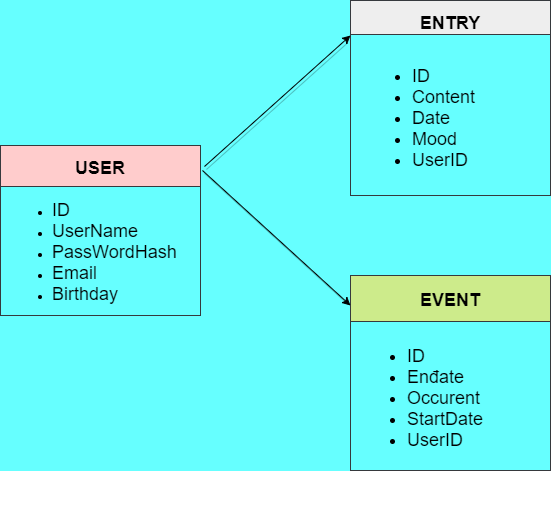
\includegraphics[height=140pt,width=240pt]{Images/h1.png}
	  \caption{Cở sở dữ liệu trong hệ thống.}
	  \label{mainbook1}
	 \end{figure}


Như hình \ref{mainbook1} ta thấy dữ liệu gồm có 3 phần chính: người dùng (USER), nhật ký (ENTRY), các sự kiện (EVENT).


\begin{itemize}
	\item Người dùng (USER) : có 4 trường dữ liệu chính. Trong đó ID của từng người dùng sẽ là khác nhau và được sinh tự động. Trường ID của mỗi người dùng sẽ là khác nhau, do đó, ta có thể phân biệt từng người dùng với nhau thông vào trường này. Hơn nữa, trường ID này cũng là khóa chính để tham chiếu đến trường ENTRY và EVENT. Các trường còn lại do người dùng nhập vào khi thực hiện thủ tục đăng ký.

	\item Nhật ký (ENTRY) : ENTRY lưu trữ các thông tin của người dùng. Hãy tưởng tượng với trang facebook. ENTRY này sẽ lữu trữ các cảm nghĩ, hình ảnh, video,... mà mỗi khi bạn upload lên.

	\item Sự  kiện (EVENT) : EVENT lưu trữ những thông tin mà ta đã đặt hẹn trước. Event này cũng có thể là một sự kiện báo ngày sinh nhật, đặt lịch hẹn...

\end{itemize}


\subsection{Thiết kế các khối chức năng và hệ thống con}

\begin{figure}[!h]
	  \centering
      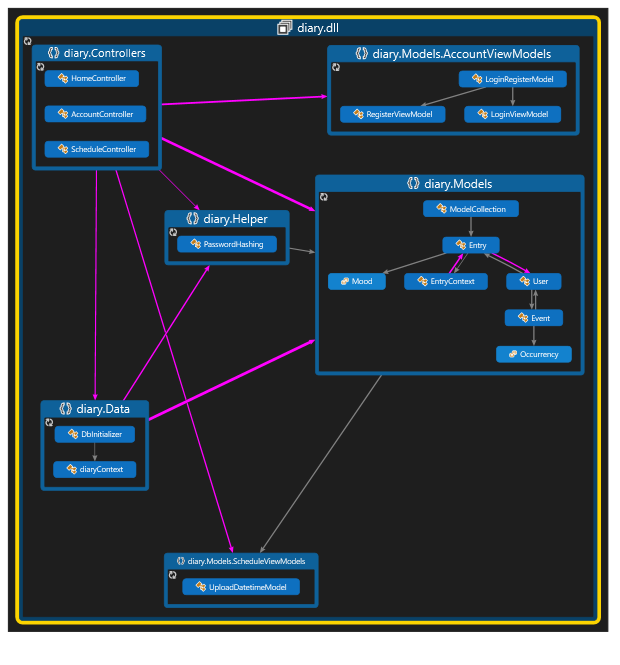
\includegraphics[height=365pt,width=320pt]{Images/h2.png}
	  \caption{Sơ đồ lớp của hệ thống.}
	  \label{mainbook2}
	 \end{figure}

Như hình \ref{mainbook2} phần mềm chúng ta thực hiện theo mô hình MVC với kiến trúc gồm 3 phần chính Controller - điều phối, Model - tạo dữ liệu, View - để hiển thị. Cùng với đó là các phần phụ khác để hỗ trợ.


\begin{enumerate}
	\item \textbf{Model}

			\begin{figure}[!h]
	 			\centering
      			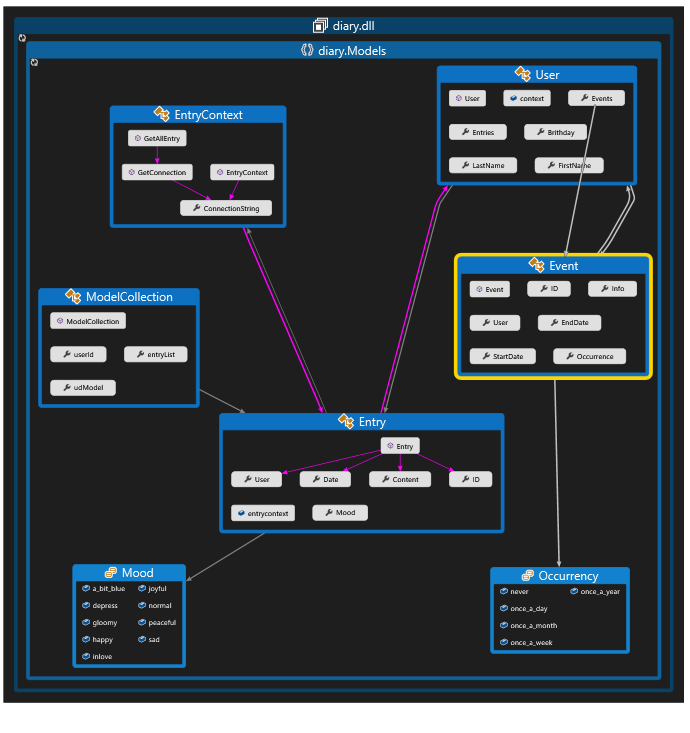
\includegraphics[height=480pt,width=440pt]{Images/h4.png}
	 		 	\caption{Mô tả Model 1}
	 		 	\label{mainbook3}
	  		\end{figure}


	  \newpage


		\begin{figure}[!h]
	  \centering
      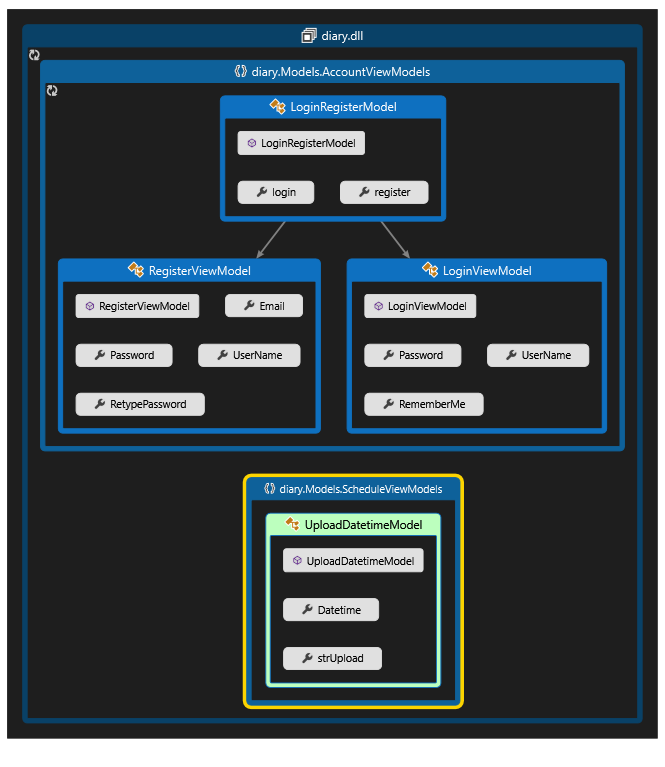
\includegraphics[height=460pt,width=400pt]{Images/h5.png}
	  \caption{Mô tả Model 2}
	  \label{mainbook4}
	   \end{figure}


	Đối với Model ta có 3 trường dữ liệu chính : User, Entry và Event. Ngoài ra, còn có thêm trường ErrorViewModel và ModelCollection (hình \ref{mainbook3} \& hình \ref{mainbook4})

	\begin{itemize}
		\item \textbf{User} : như đã biết user này chứa thông tin của một người dùng như tên, Ngày sinh,... và được tham chiếu đến Entry và Event.
		\item \textbf{Entry} : Trường này chứa nội dung nhật ký mà người dùng muốn lưu. Context sẽ chứa nội dung nhật ký, Date chứa ngày lưu nhật ký ... Có thêm một enum mood về cảm nghĩ khi viết nhật ký đó.

		\item \textbf{Event} : Trường này lưu trữ các sự kiện sẽ diễn ra và thông báo cho người dùng biết. StartDate sẽ lưu trữ ngày cập nhật sự kiện, EndDate lưu trữ ngày thông báo sự kiện ... Có thêm trường Occurrence để mặc định khoảng thời gian thông báo sự kiện.



	\end{itemize}

			Ngoài ra trường ErrorViewModel hiển thị error khi có lỗi xảy ra. Còn ModelCollection là cấu hình các dữ liệu chứa trong model để truyền vào View. \\

			Ta cũng còn hai Model chính để cấu hình dữ liệu để thực hiện các thủ tục. (hình \ref{mainbook4})

			\begin{itemize}
				\item \textbf{LoginRegisterModel} : Model này giúp ta thực hiện thủ tục Đăng nhập, Thoát và đăng ký tài khoản. Nó sử dụng hai Model RegisterViewModel và LoginViewModel. Lưu ý rằng, khi đăng nhâp hoặc đăng ký thì tài khoản sẽ được hash thông qua hàm hash trong Mục Help sẽ nói sau.

				\item \textbf{ScheduleViewModel} : Model này có tác dụng lưu dữ liệu cho các hoạt động hiển thị của người dùng.



			\end{itemize}


	\item \textbf{Controller}

		Controller sẽ thực hiện việc điều phối của Model sang View. Phần mềm có 3 controller chính HomeController, AccountController, ScheduleController. (hình \ref{mainbook5}). Phần mềm có sử dụng Identity FrameWork để nhận biết xem người dùng đã đăng nhập chưa và người dùng đang sử dụng là ai.

	\begin{itemize}
		\item \textbf{HomeController} : Trang Home là giao diện chính của phần mềm được điều phối thông qua HomeController. Controller này có nhiệm vụ trả về một biến ngày tháng năm hiện tại và được sử dụng sau.

		\item \textbf{AccountController} : Khi người dùng chọn sign in thì Controller này sẽ xử lý. Thông qua UserManager và SigninManager, phần mềm biết được người dùng này là ai và đã đăng nhập hay chưa. Nếu chưa đăng nhập sẽ đưa đến trang đăng nhập nếu đã đăng nhập rồi thì đưa đến trang Schedule của người dùng hiện thời.

		\item \textbf{ScheduleController} : sau khi đăng nhập đúng thì Controller này sẽ xử lý. Nhờ vào DbContext để lấy dữ liệu từ database và Identity để hiển thị chính xác dữ liệu cần mong muốn.

	\end{itemize}

	\item \textbf{View}
		Phần này dùng để hiển thị. Sử dụng một số ngôn ngữ về front-end như : html, css,  javascript, jquery. Đặc biệt với ASP.NET có một kiểu trang là Razor, định dạng cshtml và có thể viết code \(C\#\) chung để hiển thị dữ liệu song song với một trang web tĩnh. Đây được coi là một file xử lý bên client side, dữ liệu sẽ được truyền vào và client sẽ xử lý để hiển thị dữ liệu ra theo lập trình.

	\item \textbf{Các phần Khác - hình \ref{mainbook6}}
	Ngoài ra, phần mềm cũng có thêm một số hỗ trợ như Xây dựng dữ liệu thông qua diaryContext. Hash mật khẩu thông qua hàm HashPassword, kiểm tra xem mật khẩu đó có đúng hay không thông qua VerifyHashedPassword. Để Hash mật khẩu phần mềm dùng kỹ thuật SHA1 của thử viện Crytography.

	\newpage


			\begin{figure}[!h]
	 			\centering
      			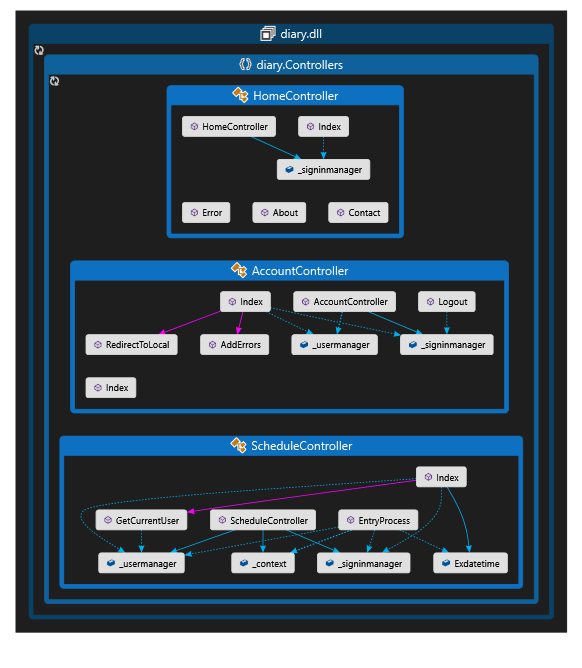
\includegraphics[height=500pt,width=440pt]{Images/h3.png}
	 		 	\caption{Mô tả Controller}
	 		 	\label{mainbook5}
	  		\end{figure}


	\newpage


	\begin{figure}[!h]
	 			\centering
      			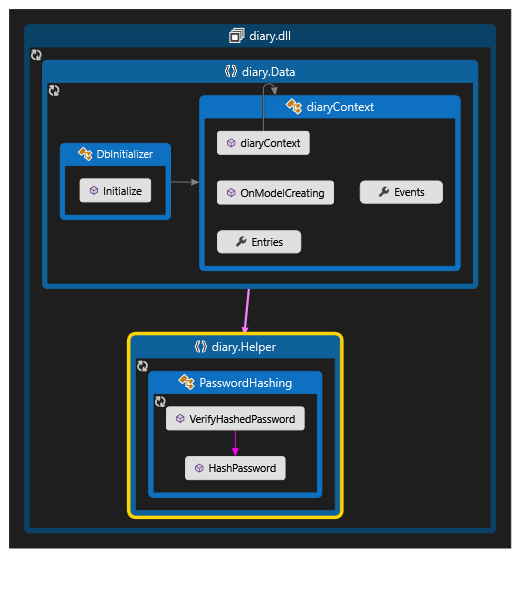
\includegraphics[height=440pt,width=390pt]{Images/h6.png}
	 		 	\caption{Mô tả các phần khác}
	 		 	\label{mainbook6}
	  		\end{figure}
\end{enumerate}


	\newpage


\subsection{Thiết kế giao diện và use case}

\begin{enumerate}
	\item \textbf{Thiết kế giao diện}

	\begin{figure}[!h]
	 			\centering
      			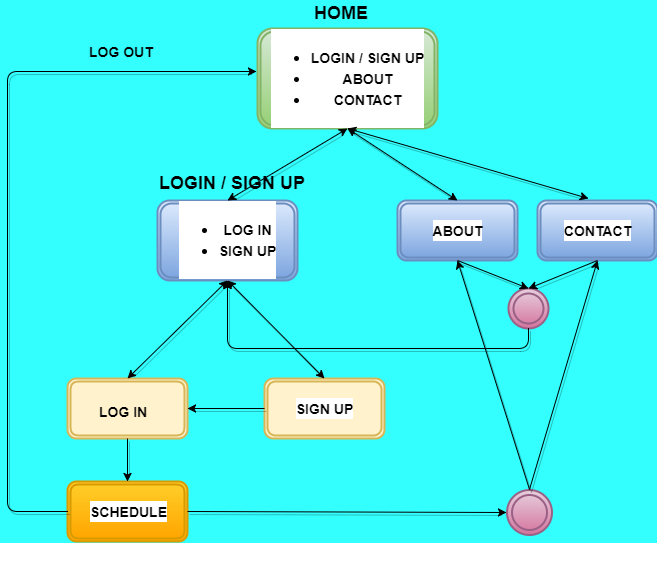
\includegraphics[height=310pt,width=300pt]{Images/h7.png}
	 		 	\caption{Mô Phỏng giao diện}
	 		 	\label{mainbook7}
	  		\end{figure}

	\begin{figure}[!h]
	 			\centering
      			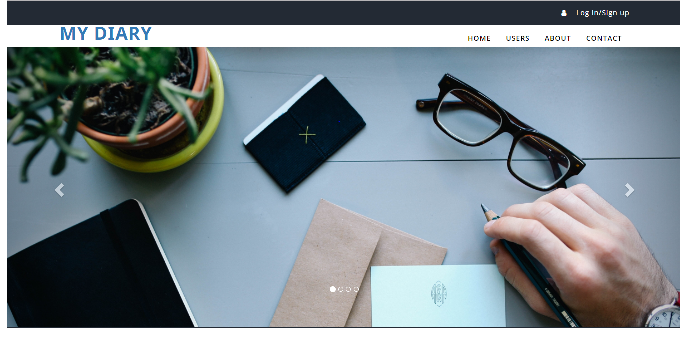
\includegraphics[height=220pt,width=410pt]{Images/h8.png}
	 		 	\caption{Home Page}
	 		 	\label{mainbook8}
	  		\end{figure}


	\begin{figure}[!h]
	 			\centering
      			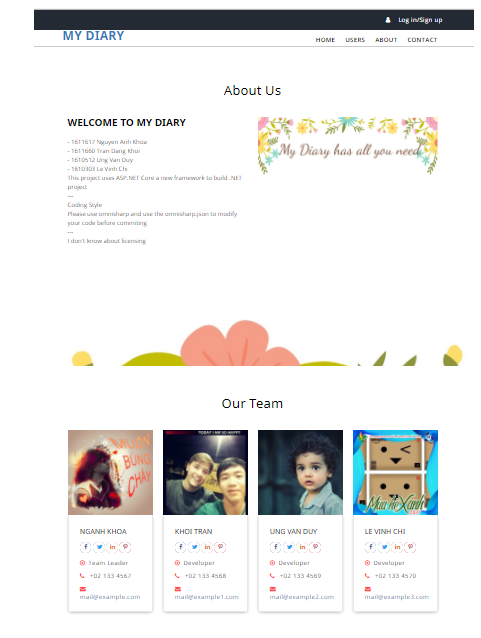
\includegraphics[height=300pt,width=240pt]{Images/h9.png}
	 		 	\caption{About Page}
	 		 	\label{mainbook9}
	  		\end{figure}


	\begin{figure}[!h]
	 			\centering
      			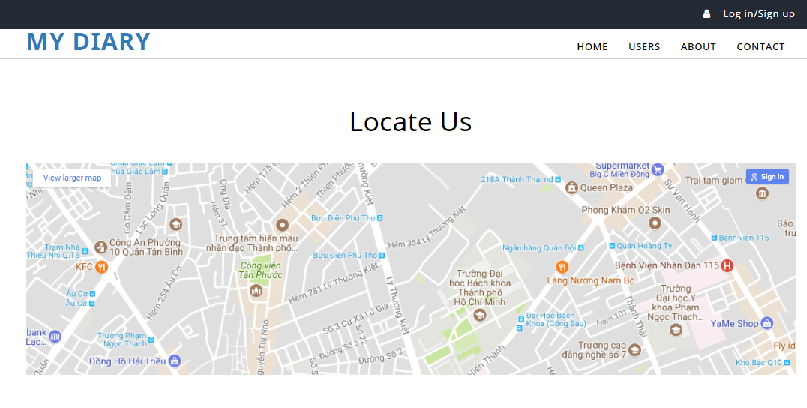
\includegraphics[height=270pt,width=310pt]{Images/h10.png}
	 		 	\caption{Contact Page}
	 		 	\label{mainbook10}
	  		\end{figure}


	\begin{figure}[!h]
	 			\centering
      			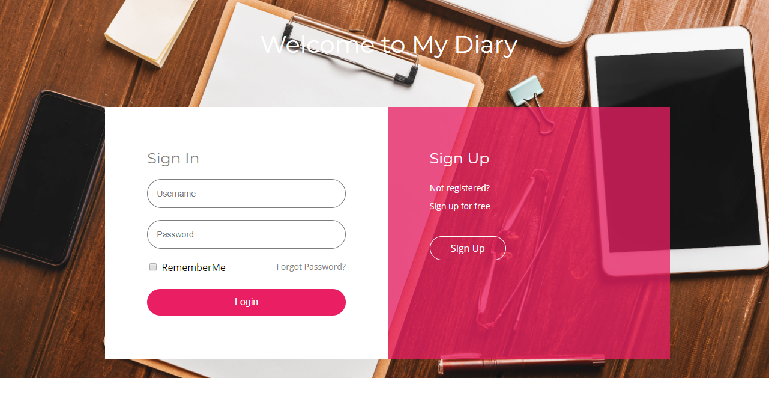
\includegraphics[height=260pt,width=380pt]{Images/h11.png}
	 		 	\caption{Login Page}
	 		 	\label{mainbook11}
	  		\end{figure}


	\begin{figure}[!h]
	 			\centering
      			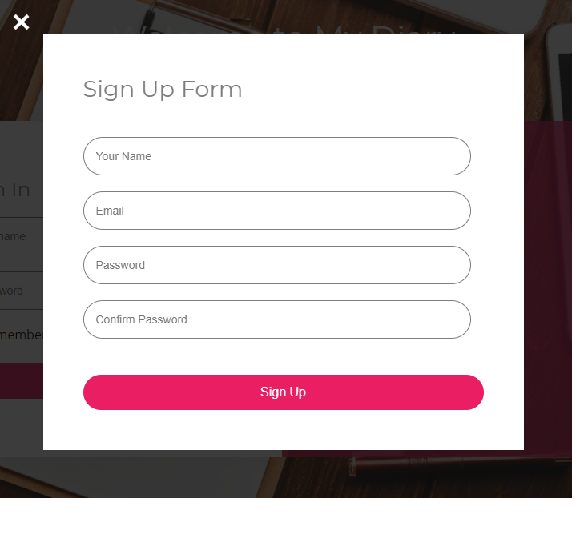
\includegraphics[height=310pt,width=340pt]{Images/h12.png}
	 		 	\caption{Sign up Page}
	 		 	\label{mainbook12}
	  		\end{figure}



	  		\begin{figure}[!h]
	 			\centering
      			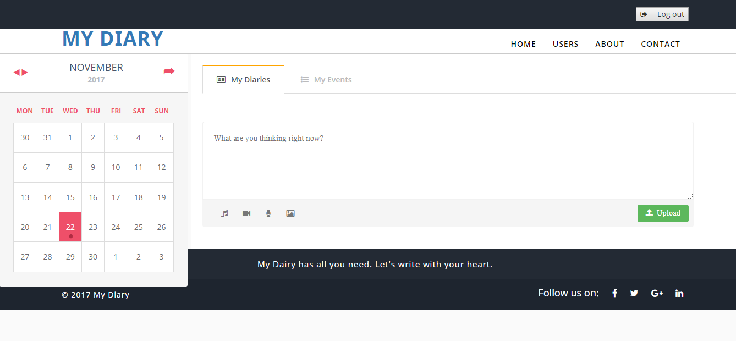
\includegraphics[height=240pt,width=470pt]{Images/h13.png}
	 		 	\caption{Schedule Page}
	 		 	\label{mainbook13}
	  		\end{figure}

	\item \textbf{Use case}

	\begin{figure}[!h]
	 			\centering
      			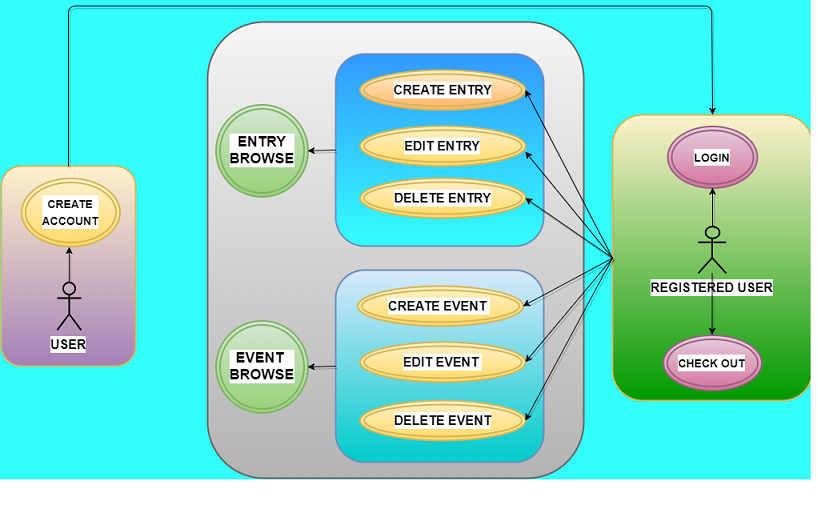
\includegraphics[height=260pt,width=450pt]{Images/h15.png}
	 		 	\caption{UseCase diagram}
	 		 	\label{mainbook15}
	  		\end{figure}


\end{enumerate}


\section{Tổ chức và quản lý mã nguồn trong quá trình quát triển}

	\begin{itemize}
		\item \textbf{Link Github} : \url{https://github.com/nganhkhoa/diary\_aspnetcore}




		\item \textbf{Sơ đồ tổ chức code}


		\begin{figure}[!h]
	 			\centering
      			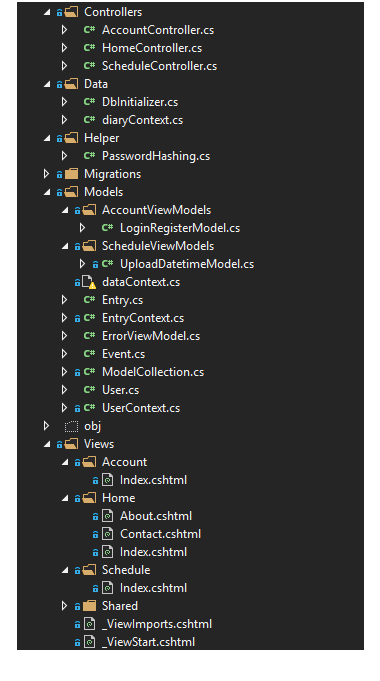
\includegraphics[height=520pt,width=300pt]{Images/h14.png}
	 		 	\caption{Sơ đồ tổ chức code}
	 		 	\label{mainbook14}
	  		\end{figure}

	\end{itemize}


\section{Các tài liệu}

\subsection{Coding style}

Sử dụng omnisharp như một công cụ để auto format code \(C\#\), sử dụng định dạng được miêu tả ở file omnisharp.json.


\subsection{Tài liệu hướng dẫn sử dụng phần mềm}

	Có lẽ mọi người đã rất quen thuộc với một trang web nhật ký. Với phần mềm diary này cũng vậy, phần mềm với giao diện dễ sử dụng giúp cho việc tiếp cận với phần mềm dễ dàng và thuận tiện. Sau đây là một số hướng dẫn cụ thể khi sử dụng phần mềm.

	\begin{enumerate}
		\item \textbf{Đăng nhập và đăng ký}
		Khi sử dụng phần mềm người dùng đầu tiên sẽ được làm việc với trang chủ hệ thống (như hình \ref{mainbook16} ).

		\begin{figure}[!h]
	 			\centering
      			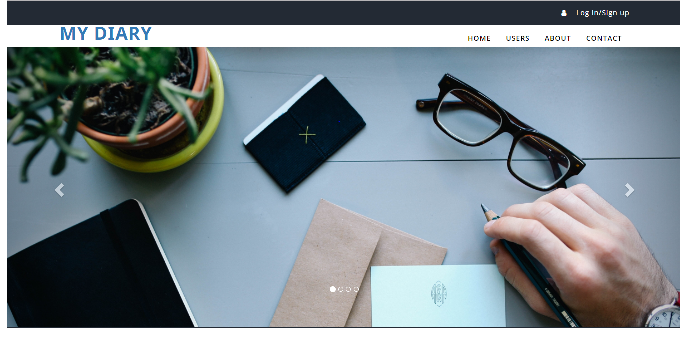
\includegraphics[height=250pt,width=340pt]{Images/h8.png}
	 		 	\caption{Home Page}
	 		 	\label{mainbook16}
	  		\end{figure}

		Để \textbf{Đăng ký} hoặc \textbf{Đăng nhập} vào hệ thống người dùng phải :


			\begin{itemize}
				\item Nhấn chọn Login/Sign up ở góc trên bên phải trang chủ.
				\item Sau đó, một trang đăng nhập/đăng ký sẽ hiện ra (như hình \ref{mainbook17})

				\begin{figure}[!h]
	 			\centering
      			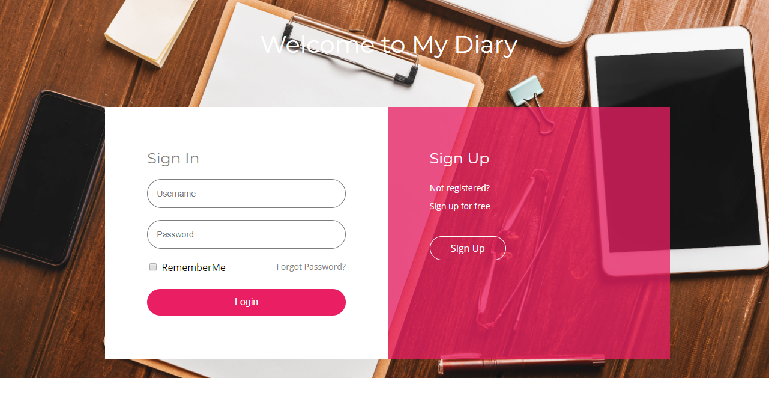
\includegraphics[height=250pt,width=340pt]{Images/h11.png}
	 		 	\caption{Log In/Sign Up Page}
	 		 	\label{mainbook17}
	  		\end{figure}

				\item Nếu muốn \textbf{Đăng ký} một tài khoản, ta nhấn chọn \textbf{Sign Up}, một form Sign Up sẽ hiện ra yêu cầu nhập vào các trường thông tin cần thiêt (như hình \ref{mainbook18}). Sau khi đã điền đầy đủ chọn sign up ở góc dưới Form. Nếu thông tin là hợp lệ thì sẽ chuyển đến trang Login cho người dùng đăng nhập vào hệ thống, ngược lại, chương trình sẽ hiển thị lỗi để người dùng biết và nhập lại.

				\begin{figure}[!h]
	 			\centering
      			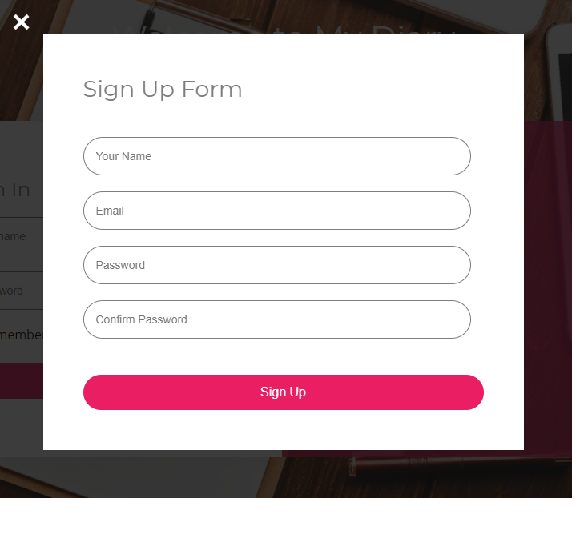
\includegraphics[height=200pt,width=270pt]{Images/h12.png}
	 		 	\caption{Sign Up Form}
	 		 	\label{mainbook18}
	  		\end{figure}

				\item Sau khi đã có trong tay một tài khoản hợp lệ, người dùng có thể chọn điền vào các trường UserName và Password để đăng nhập và chọn \textbf{Log In} để đăng nhập vào hệ thống.

			\end{itemize}


\newpage

		\item \textbf{Sử dụng các tính năng}
			\begin{enumerate}
				\item \textbf{Tạo, hiệu chỉnh \& xóa Entry }


			\begin{itemize}

				\item Sau khi đã Login thành công, lúc này người dùng đang ở trang Schedule của mình. (như hình \ref{mainbook19} )

				\begin{figure}[!h]
	 			\centering
      			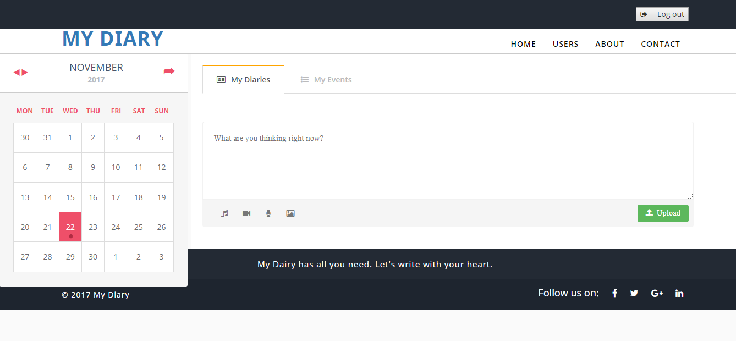
\includegraphics[height=200pt,width=320pt]{Images/h13.png}
	 		 	\caption{Schedule Page}
	 		 	\label{mainbook19}
	  		\end{figure}


				\item Để \textbf{Tạo} mới 1 Entry, người dùng có thể điền thông tin vào Textbox  rồi nhấn \textbf{Upload}. Khi đó, một Entry mới sẽ xuất hiện ở khung bên dưới. Người dùng cũng có thể chọn Emotion (biểu cảm khi đăng entry đó) hay tùy chỉnh trên thanh \textbf{Upload} chọn hình ảnh, video để Upload lên.

				\item Để \textbf{Hiệu chỉnh} 1 Entry, người dùng cần đi đến Entry cần hiệu chỉnh chọn biểu tượng \textbf{Cây bút}, một Form yêu cầu nhập thông tin cần hiểu chỉnh. Sau khi nhập xong chọn \textbf{Update} để hoàn thành.

				\item Để \textbf{Xóa} 1 Entry, thực hiện tương tự như \textbf{Hiệu chỉnh vậy} nhưng thay vì chọ biểu tượng \textbf{Cây bút}, hãy chọn biểu tượng \textbf{Thùng rác}.

				\end{itemize}
		Người dùng cũng có thể chọn thời gian ở lịch bên trái, khi muốn xem những Entry ở ngày đó.

				\item \textbf{Tạo, hiệu chỉnh \& xóa Envent}

			\begin{itemize}
				\item Để đặt các event người dùng cần nháy vào nút \textbf{MyEvent} để chuyển sang trang này.
				\item Nhập thông tin của sự kiện vào ô Textbox sau đó đặt thời gian bắt đầu và kết thúc của sự kiện ở ô bên dưới. Chọn \textbf{Upload}. Một Event mới sẽ được xuất hiện.
				\item Các thao tác \textbf{Hiệu chỉnh \& Xóa} một Event tương tự như với Entry vậy.

			\end{itemize}
				Người dùng cũng có thể chọn thời gian ở lịch bên trái, khi muốn xem những Event ở ngày đó.

			\end{enumerate}


	\end{enumerate}




%%%%%%%%%%%%%%%%%%%%%%%%%%%%%%%%%
\addcontentsline{toc}{section}{Tài liệu tham khảo}
\begin{thebibliography}{99999}
\bibitem[tvtt]{tvtt} {Web Diary : \url{http://bkudiary.azurewebsites.net/}}. Trang web được host lên.
\bibitem[tvtt]{tvtt} {Web Diary : \url{https://github.com/nganhkhoa/diary_aspnetcore/releases}}. Phiên bản release của chương trình.
\bibitem[tvtt]{tvtt} {Web Diary : \url{https://www.useloom.com/share/e841829586af48239801d4e0c21a4cb7}}. Video demo chương trình.



\end{thebibliography}
\end{document}

